\Chapter{A keretrendszer tervei}

\Section{Osztályok és kapcsolataik}

A keretrendszer a széles körben elterjedt objektum orientált tervezési módszereknek megfelelően készült. Az alkalmazáshoz tartozó osztályok és azok kapcsolatai \aref{fig:UML}. ábrán láthatók.

\begin{figure}[!ht]
    \centering
    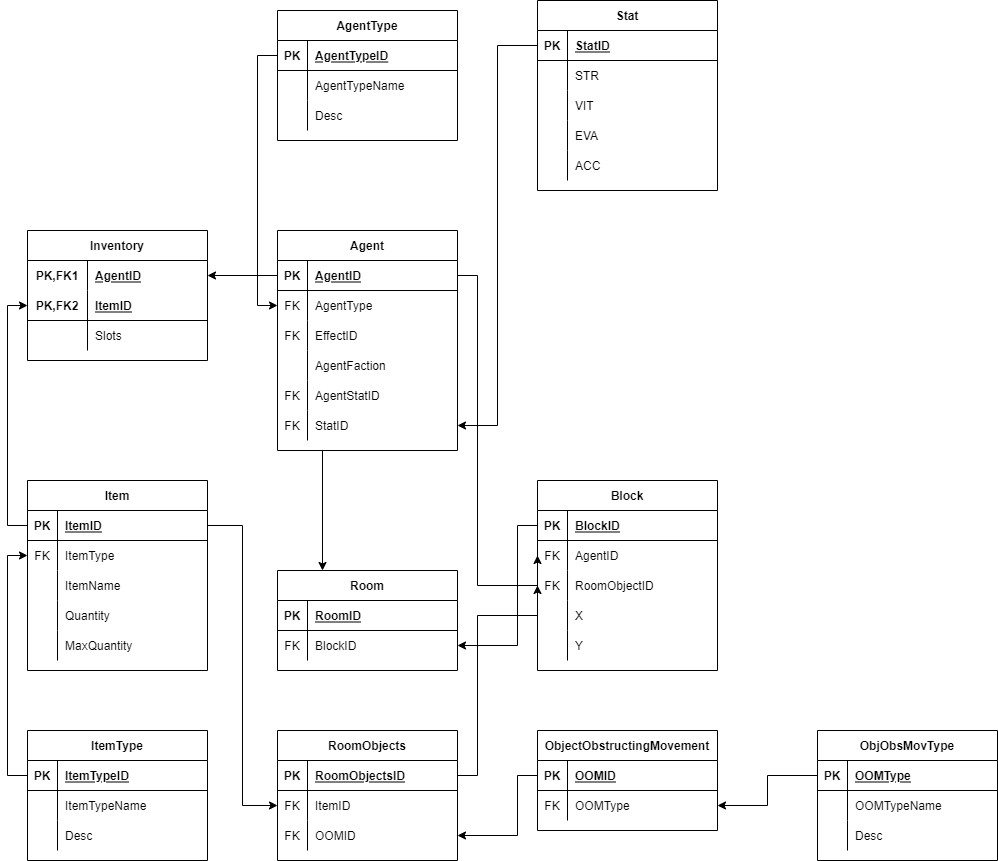
\includegraphics[width=\textwidth]{images/relaciosadatmodel7.png}
    \caption{Legelső tervezéshez tartozó relációsadatmodel}
    \label{fig:relmod}
\end{figure}

\newpage

A tervezési és specifikálási fázis elején megtervezett első relációs model látható a \ref{fig:relmod}. ábrán.

Először az ágensekhez tartozó statisztikák és az \textit{Inventory} került bele az ágensek adataiba.

A szobák fogalma nem valósult meg, nincsenek meghatározva mely blokkok alkotják egy adott szobát.

A szobákban lévő objektumok végül úgy lettek megoldva, hogy a térképen vannak elhelyezve koordináta alapján. És a hozzátartozó típusok is az objectbe kerültek.

Az ID használata nem valósult meg a megvalósítás részben, illetve nem tartalmazta még a játékmenetet irányító osztályokat se.

\begin{figure}[!ht]
    \centering
    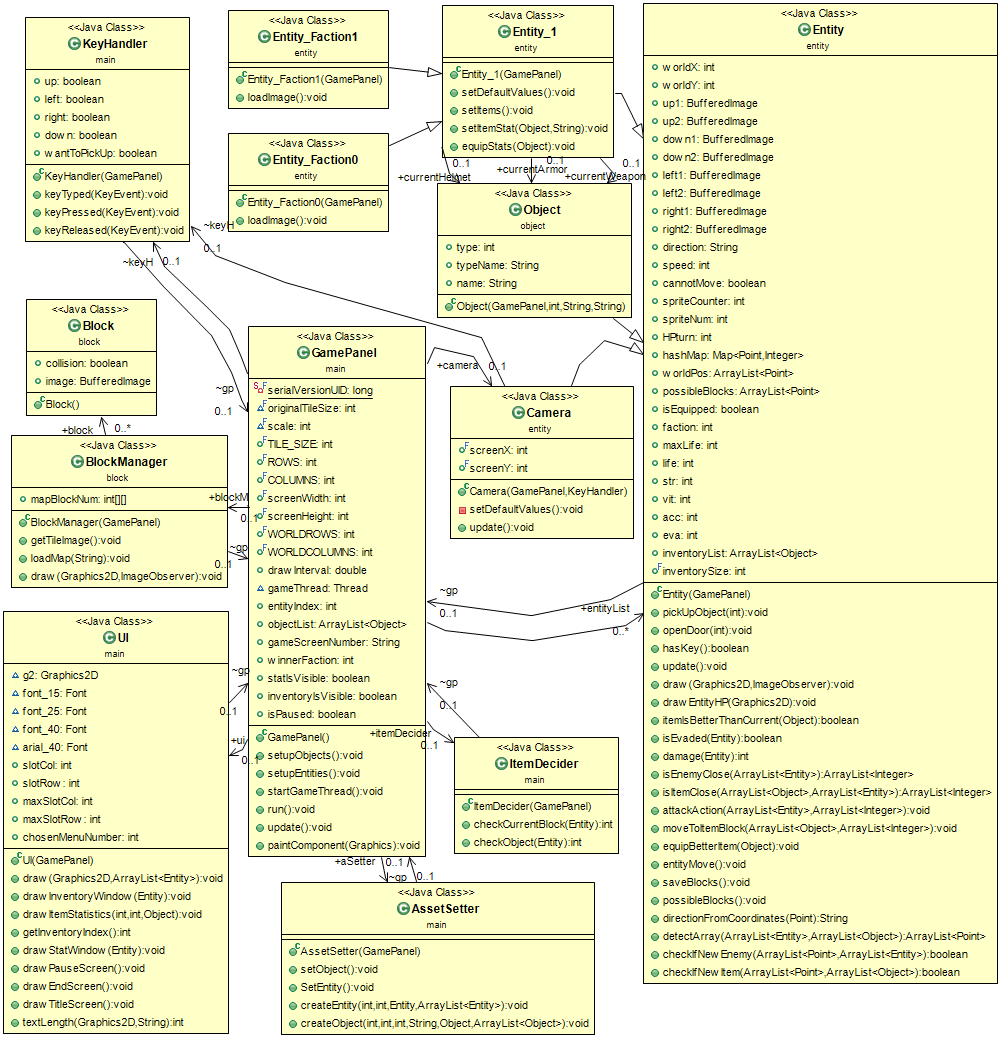
\includegraphics[width=\textwidth]{images/UML.png}
    \caption{A keretrendszerhez tartozó osztályok}
    \label{fig:UML}
\end{figure}

\noindent A következő szakaszok részletesen kitérnek ezek szerepére.

\subsection{KeyHandler}

A KeyHandler osztály felel a kamera mozgatásáért, a játékmenet megállításért/elinditásáért, UI elemek használatáért, 
mint például az Inventory és Statistics oldal megnyitása/bezárása.

\subsection{Block}

Blockok néhány változóit tartalmazza.

\subsection{BlockManager}

\textit{Block} típusok definiálása, tulajdonságok megadása és képek beolvasása a res mappából.

Egy txt file-ból beolvas egy $50 - 50$-es mátrixot, amelyben minden elem egy 0, 1 vagy 2. Az elemek szóközzel vannak elválasztva.

Megrajzolja a térképet megvalósító blokkok kinézetet az alapján, hogy hol helyezkedik el a térképen és hogy milyen blokk kép tartozik a blokk típusához.

\subsection{GamePanel}

Tartalmazza a képernyő adatokat, és a blokkok méretét, az ágens listát és az objektumok listáját.
Itt inicizálódik a kezdő képernyő az alkalmazás elindítása után.
Tartalmazza azokat a függvényeket, amelyek tartalmazzák az ágens és objektum létrehozását, ezek hívódnak meg a \textit{main}-ben.
Felelős a \textit{UI} elemek, az ágensek és tárgyak megrajzolásáért.

\subsection{Camera}

Kamera kezdő helyzetét, lépés távját határozza meg.
Meghatározza a képernyő koordinátáit is.

\subsection{AssetSetter}

Az objektumok és ágensek elhelyezésért felelős.
Két fontosabb függvényt tartalmaz, amelyek felelősek az ágensek és a térképen minden megtalálható objektum létrehozásáért a szimuláció elején.

\subsection{UI}

A gameScreenNumber változó által tárolt 3 fő képernyő megjelenítését tartalmazza: Kezdő képernyő(title),
játékmenet(normal) és végsőképernyő(end).
Itt történnek a képernyőre való szöveg kiírások is.
Inventory és Statistics ablak megjelenítését is tartalmazza.

\subsection{Entity}

A következő fontosabb ágens adatok tárolja:
\begin{itemize}
    \item $X$ és $Y$ koordináta: a térképen lévő helyzetét jelentő értékek
    \item \textit{HPturn}: Azt az érték tárolja, hogy hány kör múlva lesz életerő regenerálódás.
    \item Alapstatisztikák: Életerő, erő, kitartás, kitérés, pontosság.
    \item \textit{InventorySize}: Az \textit{Inventory}-ban maximálisan elhelyezhető objektumok száma.
    \item Irányát: Meghatározza, hogy melyik irányba néző képet kell betöltenie.
    \item Gyorsaság: Lépésenként mennyi utat tesz meg, ez egy rögzített érték, amely egy blokknyi távolság.
\end{itemize}

\noindent Itt történik az ágensek :
\begin{itemize}
    \item életcsíkjának a megrajzolása,
    \item megrajzolása a képernyőre,
    \item által legutoljára felvett hordható tárgy statisztika vizsgálata,
    \item tárgy felvétele,
    \item támadása, kulcs használata és mozgása,
    \item találatának eldöntése és sebzés méretének a kiértékelődése,
    \item és objektumok észlelése,
    \item \textit{hashMap} értékeinek frissítése.
\end{itemize} 

\subsection{ItemDecider}

Két fontosabb függvényt tartalmaz, amely egy-egy indexet ad vissza az Entity osztálynak, amelyek által kiértékelődik az ágensek következő lépései.
Az egyik függvény azt vizsgálja, hogy van-e valamilyen objektum az ágens koordinátáján, a másik függvény azt vizsgálja, hogy van-e az ágens koordinátája
alatti, feletti, jobb oldali vagy baloldali szomszédján valamilyen object.

\subsection{Object}

Az objectek osztálya, object típusokat tartalmaz.
Az objectek típusát, típus nevét és nevét tárolja.
Ezek származtatásával jönnek létre az objectek a térképen.

\subsection{Entity1}

Ágensek egyetlen típúsának alap értékeinek definiálására szolgál.
Tartalmazza az ágensek kezdő felszereléseit, ezeknek a felszereléseknek a változói itt kapnak értéket.
És itt kerülnek felszerelésre az ágensre statisztikailag és kerülnek be az \textit{Inventory}-ba.

\subsection{EntityFaction1}

A faction 1-hez tartozó ágensek képeit tárolja, amelyeket láthatunk a szimulációban.

\subsection{EntityFaction0}

A faction 0-hez tartozó ágensek képeit tárolja, amelyeket láthatunk a szimulációban.


